\documentclass{book}
\usepackage{xeCJK}
\usepackage{graphicx}
\usepackage{amsmath}

\begin{document}
\title{Systems and Software Verification中文翻译版本}
\author{林奇峰}
\date{\today}
\maketitle
    \chapter{Automata 自动机}

    正如前言所述,模型检查包括验证系统模型的一些属性。在任何检查开始之前,一个人就必须面对正在研究的系统的建模任务。坦白地说,我们强调这个建模步骤是困难的,但又对后续获得的结果的相关性至关重要。没有通用的方法来建模一个系统:建模是一项具有挑战性的任务,最后交付给一些能够很好结合物理现实和应用现实或者计算机模型的资深工程师来执行。此外,在建模前引入建模专家和“区域”专家的混合团队的做法是可取的。

    这一章并不是说能提供一种极其简单的建模方法(不然,不夸张地说是这是过于雄心勃勃的目标)。相反地,我们会谦虚地为大多数模型检查方法提供一种通用基础模型来破除迷惑或者其他阻碍。在本章中使用玩具示例,我们将说明这个通用模型是如何用来表示对象或“真实的”系统的。

1.1 引导例子(Intoductory Examples)

    最适合用模型检查技术来验证的系统是那些容易被(有限)自动机们建模的系统。简单地说,自动机是一种利用转换(transition)操作来从一个状态(state)迁移到另外一个状态的机器。例如,一个数字手表可以用一个自动机来表示。当中,每个状态代表了当前的小时和分钟(我们忽略了秒)。因此有24 x 60 = 1440个可能的状态。而且任意一个状态对有一条转换链。状态保存了一分钟过去的当前时间
    \begin{figure}
    \centering
    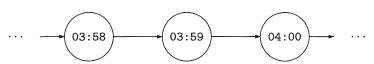
\includegraphics[height=0.6in,width=4.0in]{1_1.jpg}
    \caption{A model of watch}
    \end{figure}

    自动机(或自动机的一部分)的图形化表示通常为:每个状态都是一个圆圈,每个转换都是一个箭头(见Figure 1.1)。一个没有来源的传入箭头标识初始状态。

    图形化表示的可用性是基于自动机的形式主义的优点之一。这些表示为我们理解系统操作提供了宝贵的支持。

    另一个例子(一个可以完整表示的例子,见Figure 1.2)是一个模3计数器。该自动机表示为$A_{c3}$(上面的数字表可以被看作是某种形式的1440计数器)。$A_{c3}$的状态对应于可能的计数器值。它的转换反映了在计数器上可能的操作。在这个示例中,我们将操作限制为增量(inc)和减量(dec)。
    \begin{figure}
    \centering
    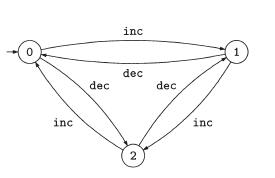
\includegraphics[height=2.0in,width=3.0in]{1_2.jpg}
    \caption{$A_{c3}$: A modulo 3 counter}
    \end{figure}


    同样的道理,一个整数变量可以建模成一个拥有无限多个状态(每个可能值对应一个)的自动机。它允许每个基本操作(肯定是递增/递减1,但也可能是一个符号更改或平方)对应一个转换。虽然存在着对拥有无限多个状态的受限自动机的模型检查技术,但这种技术在本书中只会间接提到。因此,我们从这里假设,除非我们特别提到,否则一个自动机的状态和转换是有限的。

    现在再来考虑一个稍微复杂一点的例子,例如那些控制办公室或建筑大门开/关的数码密码  (digicode)。门在键入正确的字符序列后打开,(在这个简单的数码模型中)无关于任何可能的错误初始尝试。简单起见,我们假设有3个可用的键:A, B, C,而且每当ABA被键入时,门就会打开。由此产生的数码密码可以建模成Figure 1.3所示的拥有4 种 状态和9种转换的自动机。注意图中的单个箭头有时怎样表示两个转换具有相同的起点和相同的终点(例如从3到1,或者从1到1,其中一个标记为B,另一个标记为C)。

    数码密码示例将用于说明两个基本概念,即系统模型的执行(execution)和执行树(execution tree)。执行是描述系统可能演进的状态序列。因此,第1121、12234和112312234是数码密码的执行。在某些情况下,它有利于拼出从一个状态到另一个状态的转变。因为执行1121时,从1到1的时候我们不能告知哪个键被输入【注:从1到1有B,C两种键入方式,而在1→1这个结果上不能看出哪个键被按下】。虽然我们很少会需要这些额外的信息。事实上这没有增加概念上的困难且被大多数模型检查工作所排除在外。

    我们还将关心系统的所有可能的执行。描述此集合的一种方法是按某些顺序“排列”执行(例如按照长度增加的顺序)。接着,数码密码就会表现为

    1

    11,12

    111,112,121,122,123

    1111,1112,1121,1122,1123,1211,1212,1221,1222,1223,1231,1234
    \begin{figure}
    \centering
    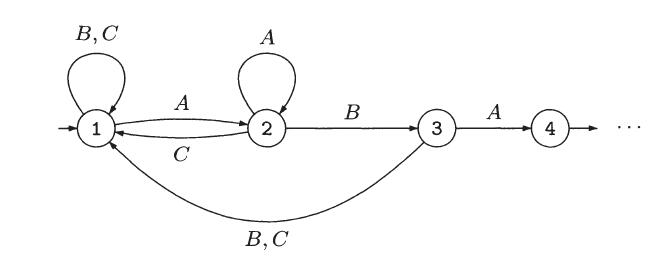
\includegraphics[height=2.0in,width=3.0in]{1_3.jpg}
    \caption{A model of a digicode}
    \end{figure}

    出于厘清的原因,我们更倾向于以树的形式组织执行集合。在计算机科学中,树的根在顶部。在这里,根是初始状态1。它的子节点(我们说的直接继承者),是在一个步骤结束后可以到达的所有状态,在我们的例子中就是1和2。我们重新开始,第1和第2节刚刚创建,分别有两个孩子分别为1和2,三个孩子分别为1、2和3。我们最终获得了一组系统执行的表示(通常是无限的)(见Figure1.4)。

    由于我们的目标是验证系统属性,或者更准确地说,为了验证系统模型的属性,我们将许多我们已知满足的基本属性与每个自动机状态关联起来。举个例子,“门是开的”的属性;存在于状态4而不存在于状态1,2,3。在我们的数码密码例子中,我们的主要兴趣是以下知识:

    1 .如果门打开了(如果执行到达状态4),那么A,B,A是最后三个按照顺序键入的字母。

    2。键入任意以ABA结尾字母序列就打开了门(也就是说,定义了通向状态4的执行)。

    建模过程中的一个关键步骤是自动机的构建。它表示了当下考虑的系统并在其中我们可以将每个状态与一些我们已知真假的基本属性关联起来。我们随后必须学会用这些基本属性和我们希望系统满足的更复杂的属性来表达自动机。用基本属性表示“复杂”属性的方法取决于我们使用的逻辑(logic)。下一章的目标正是定义这些逻辑。为了将基本性质与更复杂的性质区分开来,在提到基本性质时,我们说成(原子)命题在给定的状态中是真或假。
    \begin{figure}
    \centering
    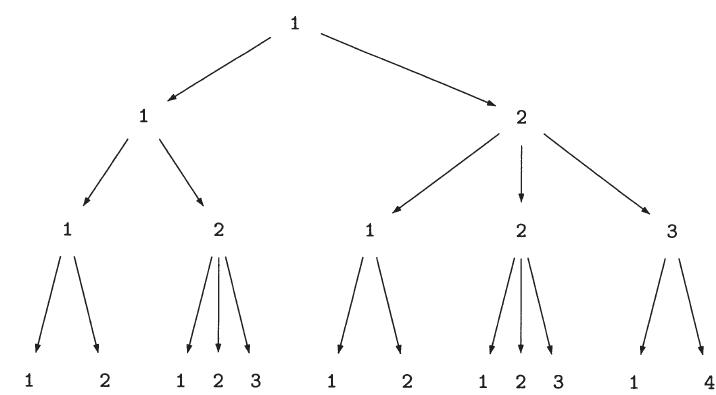
\includegraphics[height=3.0in,width=4.0in]{1_4.jpg}
    \caption{The begining of the execution tree of the digicode}
    \end{figure}

    这里我们只是简单地画出直观的想法。在我们接下来的示例中,我们可能会被引导来定义这些基本属性:
    $P_A$:刚键入A

    $P_B$:刚键入B

    $P_C$:刚键入C

    $P_A$属性存在于状态2和4,$P_B$单独存在于状态3(实际上不存在于状态1,因为按下C也可以达到),而$P_C$则不存在于任何状态。

    我们还可以定义以下属性:

    $pred_2$:执行的前一个状态为2;

    $pred_3$:执行的前一个状态是3。


    因此,$pred_2$只在状态3中保持,而$pred_3$仅在状态4中保持。现在考虑一个导致门打开的执行,即结束于状态4的执行。由于$pred_3$在状态4中保持,因此这个执行必须以序列3 4结束。但$pred_2$在状态3中保持,因此实际上执行以序列2 3 4结束。由于$P_A$存在于状态2和4,而$P_B$存在于状态3中,我们得出结论,最后三个字母键入的是A,B,A的顺序。
    因此,我们已经“证明”了两个必要的属性之一:如果门打开了,那么“正确”的字母顺序就会被键入。另一个属性以类似的方式从基本属性中获得。
    准确地来说,模型检查包含了类似这样能够使其自动运行地去验证的技术。

    \section{一些定义(A Few Definitions)}

    我们现在将简要定义上面介绍的概念。我们所称的自动机源自于语言理论的有限自动机,以及在其他领域所使用的Kripke结构({\itshape kripke structure})和转换系统({\itshape transition systems})的概念。

    {\itshape  Automata}(自动机)。给定一个基本命题的集合$Prop$= \{P1,…\},一个自动机可以表示为一个元组$\mathcal{A}=<Q, E, T, q_0, l>$

    •$Q$是状态的有限集;

    •$E$是转换标签的有限;

    •$T \subseteq Q$x$E$x$Q$的转换集合;

    •$q_0$是自动机的初始状态;

    •$l$将$Q$中的每个状态映射成该状态拥有的基本属性有限集。

    如果我们将注意力集中在Figure 1.3上的四个可见状态,那么数码密码的建模对应于以下正式的自动机定义:
    \begin{equation*}
        l=
        \begin{cases}
            1, & \mapsto{\emptyset}\\
            2, & \mapsto{P_A}\\
            3, & \mapsto{P_B,pred_2}\\
            4, & \mapsto{P_A,pred3}.
        \end{cases}
    \end{equation*}
    \begin{tabbing}
        \= $Q=\{1,2,3,4\};$ \quad   \= $T=\{(1,A,2),(1,B,1),(1,C,1),$ \\
        \> $E=\{A.B,C\}$      \> $(2,A,2),(2,B,3),(2,C,1),$\\
        \> $q_0=1$            \> $(3,A,4),(3,B,1),(3,C,1)\}$\\
    \end{tabbing}


    Graphical representation(图形化表示)。请注意,Figure 1.3并没有完全包含元组$<Q,E,T,q_0,l>$中可用的信息。实际上,为了保持原始图的简单性,没有描述出状态中原子命题的标记。我们今后将经常用出现在状态中的原子命题来表示和验证自动机。有时候由于缺少空
    间,我们会省略一些命题,或者一些状态名称。Figure1.5为数码密码示例的完整表示。类似地,我们偶尔会省略,甚至不考虑转换标签。例如当像在电子表示例中(figure1.1)这些不相关的时候。
    \begin{figure}
    \centering
    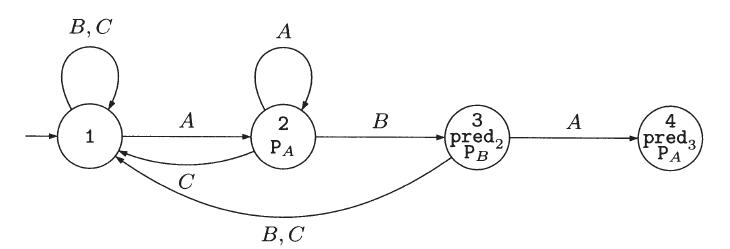
\includegraphics[height=1.5in,width=3.0in]{1_5.jpg}
    \caption{The doigicode with its atomic propositions}
    \end{figure}

    行为的正式定义(Formal defination of behavior)。自动机的路径是一个简单的,有限或者有限长的转换序列${\sigma}$。序列中的转变如$q'=q_i+1$一样一个接着一个:比如
    \begin{equation*}
    3\xrightarrow{B} 1\xrightarrow{A} 2\xrightarrow{A} 2
    \end{equation*}是一个digicode路径(见Figure 1.5)。
    $\sigma$的路径的长度,表示$|\sigma|$,是其潜在的转换的无限数量:$\sigma\in N \cup\{\omega\}$(其中N表示自然数的集合和$\omega$表示无穷)。第i个$\sigma$,写作$\sigma(i)$,是状态$q_i$经过i次转换后的结果。后者只有i<|$\omega$|才有定义。
    偏置执行(partial execution)是从初始状态$q_0$开始的一条路径。例如
    \begin{equation*}
    1\xrightarrow{A} 2\xrightarrow{A} 2\xrightarrow{B} 3
    \end{equation*}

是数码密码的部分执行代码。

    完全执行(complete execution)是一个最大的执行,即不能被扩展的执行。因此,它要么是无限的,要么结束于一个没有其他转变方式能够考虑的状态$q_n$,(在这种情况下,我们可以说成死锁)。

    当我们谈到没有限定符的执行时,我们通常指的是一个完全执行。我们偶尔会改变初始状态;我们可以通过引用“执行……””来表示。

    完全执行是自动机的真实行为;这些与活跃度的假设有关。根据这一假设,自动机总是最终完成到另一个状态的过渡。(注意我们的建模示例,从电子表开始,都经常依赖于这个假设)。

    执行树的正式的定义过于繁琐和冗长,而且不会对我们的讨论有所贡献。因此,我们只需满足于我们对这一概念的非正式处理,如上面的digicode例子。

    为了给这些定义一个结论,我们引入可到达状态(reachable state)的概念。如果一个状态出现在自动机的执行树中,或者换句话说,如果它存在于至少一种执行中,则该状态是可到达的。到目前为止,我们考虑的所有自动机的所有状态都是可到达的。我们稍后会看到,情况并非总是如此。

    \section{打印机管理器(A printer Manager)}
    再来看另一个例子,一台由两个用户共享的打印机。假设这个管理器建模的结果是Figure 1.6所给出的有限自动机。
    \begin{figure}
    \centering
    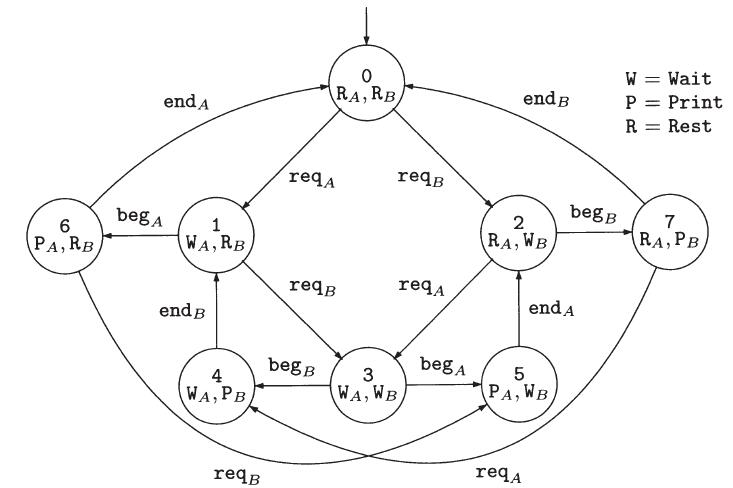
\includegraphics[height=3.4in,width=4.0in]{1_6.jpg}
    \caption{A printer manager}
    \end{figure}

    显然,最重要的是各种行为或命题的“物理”意义。$req_A$是用户A发出的打印请求,$beg_A$是一条来自打印机,暗示应开始用户A的打印作业的消息。$end_A$是一条来自打印机,暗示用户A的打印作业已经结束的消息。$req_B$,$beg_B$,$end_B$是对应的用户B的步骤。这些原子命题是根据以下实际来确定的:

    $W_A$:源自用户A且尚未被处理的请求(用户A正在等待);

    $W_B$:源自用户B且尚未被处理的请求;

    $P_A$:打印机正在为用户A打印文档;

    $P_B$:打印机正在为用户B打印文档;

    $R_A$:没有正在等待的用户A的请求(用户A在“休息”);

    $R_B$:没有正在等待的用户B的请求。

    正式的定义来说,打印管理器被建模成有限自动机$\mathcal{A}=<Q,E,T,q_0,l>$,其中:
     \begin{tabbing}
      test  \kill
      % \> for next tab, \\ for new line...
      $Q$=\{0,1,2,3,4,5,6,7\}; \\
      $E$={$req_A$,$req_B$,$beg_A$,$beg_B$,$end_A$,$end_B$}; \\
      $q_0$=0; \\
      $T$=\{(0,$req_A$,1),(0,$req_B$,2),(1,$req_B$,3),(1,$beg_A$,6),(2,$req_A$,3),\\
      \quad\quad (2,$beg_B$,7),(3,$beg_A$,5),(3,$beg_B$,4),(4,$end_B$,1),(5,$end_A$,2),\\
      \quad\quad (6,$end_A$,0),(6,$req_B$,5),(7,$end_B$,0),(7,$req_A$,4)\};\\

      \end{tabbing}
    \begin{flushleft}
      \begin{equation*}
        l=
        \begin{cases}
          0, & \{R_A,R_B\} \\
          1, & \{W_A,R_B\} \\
          2, & \{R_A,W_B\} \\
          3, & \{W_A,W_B\} \\
          4, & \{W_A,P_B\} \\
          5, & \{P_A,W_B\} \\
          6, & \{P_A,R_B\}\\
          7, & \{R_A,P_B\}.
        \end{cases}
      \end{equation*}
    \end{flushleft}



    现在打印机管理器已经完全建模好了。我们可以研究它的属性(更准确地来讲,是它的模型的属性)。例如,我们无疑希望证明任何打印操作之前都有一个打印请求。给定以上命题,对于用户A来说,就可以转化为:

1 .在任何执行中,$P_A$存在的任意一个状态都有一个$W_A$存在的状态在其前面。

    同样,我们想要检查任何打印请求最终是否得到满足,对于用户A,翻译成:

2.在任何执行中,$W_A$存在的任意一个状态都有一个$P_A$存在的状态在其后面。
    模型检查技术允许我们自动证明属性1是满意的(这也很容易“手工”完成)。

    这些技术也可以识别一个反例,证明属性2的失败。例如,要考虑执行0 1 3 4 1 3 4 1 3 4 1 3 4 1…(我们省略了标签)。因此,这个印刷管理是不公平的。因为它没有按照请求发出的顺序处理。因此打印管理器可以无限期地延迟打印文档!

    \section{更多变量(A Few more Variables)}
    当建模真实的系统时,让自动机操作状态变量(state variables)通常是很方便的。然后,我们便将控制(control)和数据(data)一份为二:“状态(state)+转变(transition)”构成了自动机的控制,而变量代表数据。

    最常见的情况是,自动机的变量只假设有限的值,要么因为这是被建模的系统的一个特性,或者因为这个限制是故意增加的(例如,为了使模型检查工具的使用成为可能)。即使从理论上的观点来看,只有有限值的变量本身就可以被自动的2所建模。这可以更方便地明确地考虑它们。

    因此,在数码密码的例子中,假设我们必须计算用户的错误数。为此,我们将添加一个初始值为0的整数变量ctr来累积错误的次数。自动机通过两种方式与变量交互:
    
    赋值(Assignment):转换可以修改一个(或多个)变量的值。因此,在数码密码例子中,错误的转换,也就是说,除了(1,a,2),(2,B,3)et(3,a,4)之外的所有转换,都会增加计数器。
    
    守卫(Guard):一个转换可以由变量的条件来保护。这意味着除非变量的条件满足,否则不能发生转换。
    
    \begin{figure}
    \centering
    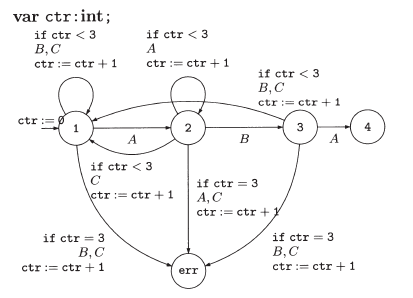
\includegraphics[height=3.4in,width=4.0in]{1_7.png}
    \caption{The digicode with guarded transistions}
    \end{figure}
    再次回到数码密码例子中,如果我们希望能够容忍用户的不超过3个错误,那么对应于错误的转换(1、B、1)、(1、C、1)、(2、C、1)等将被ctr < 3的条件所保护。然后,我们通过添加一个警报来完善系统,当检测到四个错误时发出警报。我们创建了一个新的状态err,以及从由条件ctr = 3所保护的1到err,2到err,3到err的3条转换。


    图形化表示(Graphical representation)。Figure 1.7描述了带有变量ctr的数码密码自动机。拥有guard和变量的转换根据一种已建的良好图形化传统来更新:if关键字在guard前面,然后接着转换标签,最后是赋值。为了简化,我们省略了“始终为真”的守卫,它们出现在无条件的转换上,以及没有修改任何变量的空赋值。
    
    展开(Unfolding)。例如,为了应用模型检查方法,通常需要将拥有变量的自动机的行为展开到一个只有可能的转换出现的状态图中。这样配置就可以很好被标识出来。然后我们保留着这个展开系统的“自动机”术语,即使在文章中经常会用更技术性的术语“转换系统”(transition systems)。 我们将讨论与(自动机)相关的展开自动机。
    
    展开的自动机的状态被称为全局状态(global states)。它们有许多组件:对应于“小”原始自动机A的状态,和一个给每个变量赋值的组件。我们将使用带有错误计数器的digicode的例子来说明它是如何工作的,而不是给出正式的定义。在展开之后,我们得到Figure 1.8的自动机。
    \begin{figure}
    \centering
    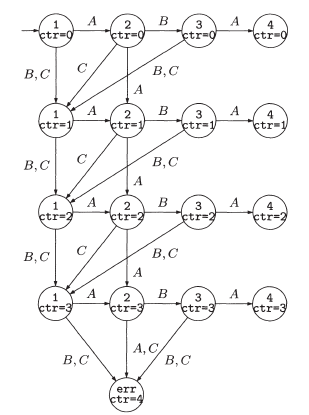
\includegraphics[height=3.4in,width=3.4in]{1_8.png}
    \caption{The digicode with error counting}
    \end{figure}

    注意转换不再被保护。因为我们明确知道每个状态下计数器的值,所以我们知道在没有guards的情况下被保护的转换是否有可能发生(在后一种情况下,根本没有转换)。
    
    还要注意,在转换过程中没有赋值。由于我们知道每个状态中计数器的值,因此一个转换直接到了新数值的全局状态。
    
    在全局状态中,例如(1,ctr = 0),我们说1是控制状态(control state)。实际上,控制状态是在其展开之前自动机的“状态”的组件。控制状态在很大程度上决定了相关的转换,尽管其作用是通过保护变量的当前值来实现的。

    \section{同步积(Synchronization Product)}
    上面的讨论显示了怎样用有限自动机为简单对象(计数器、digicode、打印机管理器等)建模。当我们处理现实中的程序或系统时,这些通常被分解成模块或子系统。为了构建整个系统的模型,很自然地,首先对系统组件进行建模。然后,通过让组件自动机进行协作来组成全局自动机。
    
    在自动机之间实现这种协作的方法有很多,即同步。在这里,我们简要介绍了主要方法。注意,用一个自动机来直接表示通常有很多状态的整个系统近乎不可能。我们称其为“状态爆炸”(stat explosion)。标准计算机可用内存能够容纳十亿个状态,而处理一个这样的作业并不罕见。
    
    一个不需同步的例子(An example without synchronization)。最简单的情况是系统可以被分解成不用相互交互的组件。全局自动机则是代表各个组件的自动机们的笛卡儿积。也就是说,一个(全局)状态实际上是由不同的组件状态(局部状态)组成的向量。
    
    例如,要建模一个由模2计数器、模3计数器和模4计数器组成的系统,我们将使用前面遇到的自动机$A_{c3}$(见Figure 1.2),我们将以类似的方式构建automata $A_{c2}$和$A_{c4}$。我们的最终系统将由3个分别有2个、3个和4个状态的自动机组成。
    \begin{figure}
    \centering
    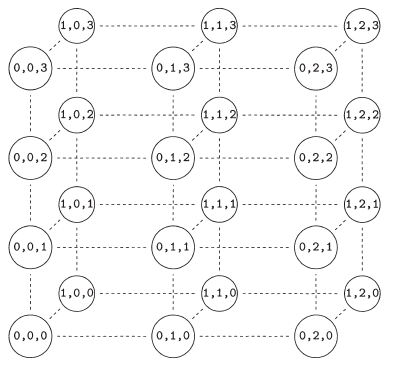
\includegraphics[height=3.4in,width=4.0in]{1_9.png}
    \caption{The states of the product of the three counters}
    \end{figure}
    全局系统自动机,表示为$\mathcal{A}_ccc$,则有2个x 3 x 4 = 24个状态。这些状态展示在Figure 1.9中。我们使用透视图来说明每个状态是如何由三个不同的组件组成的,这些组件实际上是独立的计数器。模2计数器、模3计数器、模4计数器的状态则分别在深度、宽度和高度三个维度上变化。

    我们还没有具体说明这24个状态之间的转换。事实上这些状态是从各自计数器中单独得到的。如果不需要同步,则每个状态中的每个组件(即单独计数器)都可以递减、递增或保持不变。这个结果是3×3×3 = 27个可能的选项。
    
    注意,对于单个计数器,保持不变在Figure 1.2中的没有对应的转换。这么做是为了说明在不同的计数器之间独立变化的时候计数器会怎样表现:结果是这个计数器什么事都没有做。因为这个原因,我们在27种可能性中选择忽略那些没有计数器变化的。这样在每个状态中仍然有26个可能的转变,因此在全球自动机中有24个x 26 = 624个转换。
    
    图1.10描述了初始状态0,0,0的一些转换。不用重载图表,我们只包括与一个(或更多)增量相对应的转换,并抑制任何减量的转换。这样,在26种可能性中就剩下2×2 - 2-1 = 7的转换,。从0、0、0到0、1、1被标记为“-,inc,inc”,表示第一个组件不做任何事(表示),另外两个组件执行一个inc的转换。
    \begin{figure}
    \centering
    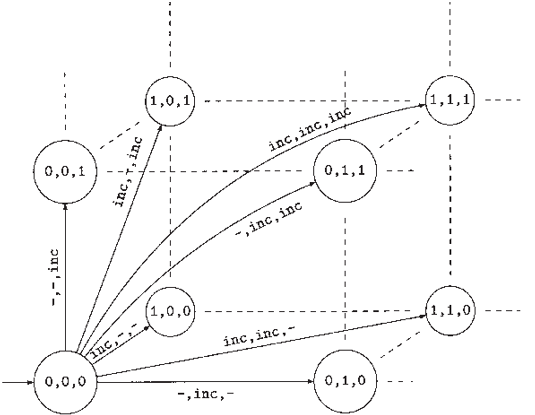
\includegraphics[height=3.4in,width=4.0in]{1_10.png}
    \caption{A few transitions of the product of the three product of the three counters}
    \end{figure}
    
    一个同步的例子({\itshape An example with synchronization})。如果我们现在想要同步三个计数器,会有很多不同的变体(选择哪个当然取决于要建模的问题的性质)。例如,我们将三个计数器绑定并且禁止其单独变化或者保持不变。则只剩下两种转换,表示为"inc, inc, inc"和"dec, dec, dec"会离开每个状态。因此只有一些状态是可达的。
    
    另一种可能,完全相反,就是将计数器解绑,同时只允许头一次在一个计数器上进行更新。则离开每个状态的转换就会单独更新一个计数器,例如“-,-,inc”以及单个计数器减量的那些。这就得到了具有24×3×2转换。我们可以也想象一个中间状态,前两个计数器同时增加或者后两个计数器同时减少。
    
    所有这些选项都很容易在一个通用的正式设置中表达为由Arnold和Nivat(AN82,Arn92)引入的自动机的同步积。
    
    同步积({\itshape Synchronization product})。让我们考虑一个有n个自动机的家族,$\forall{i}\subseteq\{ 1,…n\}$,$ A_i=<Q_i, E_i, T_i, q_0, l_i>$,并引入一个新标签“-”来表示不为任何自动机做事的虚拟动作并在组件集合的全局转换过程中保持不变。
    这些自动机们的笛卡尔积$\mathcal{A}_1$x...x$\mathcal{A}_n$就是自动机$\mathcal{A} =<Q,E,T,q_0,l>$,其中:
    \begin{itemize}
      \item $Q=Q_1$x...x$Q_n$;
      \item $E=\prod_{}{}_{1\leq i \leq n}(E_i\cup\{-\})$;
      \item $T=\left.\{ ((q_1,...,q_n),(q_1',...,q_n')) |  for\right.$ $all$ $i$, $e_i='-'$ and $q_i'=q_i$, or $e_i\neq '-'$ and $(q_i,e_i,q_i')\in T_i \left.\right\} $;
      \item $q_0=(q_{0,1},...,q_{0,n})$;
      \item $l((q_1,...,q_n))=\cup _{1\leq i \leq n}l_i(q_i)$
    \end{itemize}

    因此,在笛卡儿积中,每个组件Ai在一个转换中,要么不做任何事(虚构的动作,1'-'),要么执行“局部”转换。在不同的组件之间没有任何同步要求。此外,笛卡儿积包含所有组件“什么都不做”的转换('-')。
    
    为了同步组件,我们将限制允许在笛卡儿积中存在的转换。因此,我们定义了一个同步集(synchronization set):
    \begin{equation*}
      Sync \subseteq \prod_{1\leq i \leq n}^{}(E_i\cup\{-\})
    \end{equation*}

    Sync指明了在笛卡儿积中对应于同步(允许)的标签和那些不允许的。
    
    例如,如果我们希望将3个计数器与我们前面的示例中的3个计数器相结合,我们可以定义为同步集:Sync = {(inc,inc,inc),(dec,dec,dec)},并由一个$\mathcal{A}_{ccc}^{coup1}$(Figure 1.11)表示。
    
    
    


    同步积由自动机组件和同步集给出,也就是说,同步积的执行是源自同步集当中的笛卡儿积的执行。因此,同步积在直接积定义中可以用以下定义:
    
    $T=\left.\{ ((q_1,...,q_n),(e_1,...,e_n)(q_1',...,q_n')) | (e_i,..,e_n)\in Sync \right.$ and $\forall(i)$, $e_i='-'$ and $q_i'=q_i$, or $e_i\neq '-'$ and $(q_i,e_i,q_i')\in T_i \left.\right\} $;

    在这本书中,我们有时候用$\mathcal{A}_1||...||\mathcal{A}_n$这个表示自动机的积。隐藏的同步集必须要指明(或者保持不明)。
    
    重新标识(Relabelling)。一旦一个复杂的自动机被构造成代表子系统的许多较小的自动机的同步,就习惯在自动机积中替换一些标签。例如,在我们的计数器产品的强耦合版本中,我们倾向于简洁地写成inc而不是冗余的(inc,inc,inc)。
    
    在其他情况下,动机是不同的。例如,一旦获得了全局积,我们可能不再想要区分用于同步转换的标签和那些无关的。
    
    在这本书中,我们省略了这种重标识操作的形式(尽管是自然的,但没有信息的)定义。尽管如此,我们还是会自由地使用重新标识。
    
    可达状态(Reachable states)。判断一个同步积中的某个状态是否可达不是很显性可见。可达性当然很大程度上依赖于伴随的同步约束。例如,在三个计数器的例子中,如果我们迫使三个计数器同时变化,只有12个状态是可到达的。如果我们通过释放第三个计数器来松弛这一同步,所有24个状态将再次变得可达。然而,如果第二个计数器被释放,那么可到达的状态就是那些第一个和第三个组成部分由(0,0),(1,1),(0,2)和(1,3)所给出的,这将产生12个可到达的状态。
    
    Figure 1.11描述了我们三个计数器的强耦合积,只有从初始状态可到达的状态,以及连接这些状态的转换。每个转换都是(三元)递增或(三元)递减。
    \begin{figure}
    \centering
    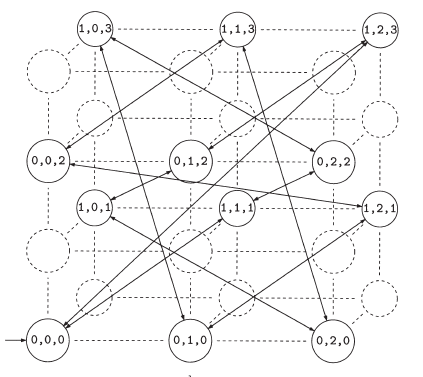
\includegraphics[height=3.4in,width=4.0in]{1_11.png}
    \caption{The automaton $A_{ccc}^{coup1}$ restricted to reachable states}
    \end{figure}
    \begin{figure}
    \centering
    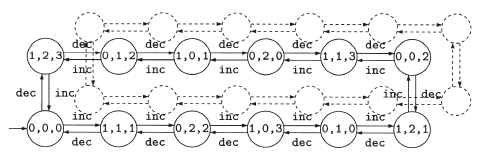
\includegraphics[height=2.0in,width=4.0in]{1_12.png}
    \caption{The rearranged automaton $A_{ccc}^{coup1}$}
    \end{figure}
    
    
    显然,一种更简单的可视化结果的方法需要自动机的空间重新调整:Figure 1.12表明,强耦合积表现为一个模12计数器。不可到达的状态用虚线表示。他们还展示了一个模12计数器的行为。
    
    接下来,我们将从给定的自动机中删除不可到达的状态得到可达图。这是与给定的自动机中唯一有关的行为描述部分。例如,通过删除图1.12中的虚线绘制的任何东西得到一个$A_{ccc}^{coup1}$的可达图。

    可达状态和验证(reachable state and verification)。当一个系统需要被验证时,我们通常会发现我们感兴趣的属性可以很简单地用可达图来标识出来的(第6章致力于可达性属性)。
   
    例如,在打印机管理器构建为同步积的情况下,我们要求两个用户同时打印的状态是可达的。
    
    为了解决这些问题,一个能够构造自动机同步积的可达图的工具将是最有用的。这本书的第三部分描述了这些工具。
    
    我们之前提到了在同步产品中确定一个状态是否可到达的困难性。这个问题实际上是可组合的。一般来说,正如后面解释的那样,任何方法都将或多或少地构建(或探索)可达图(6.3节)。这个图表的大小可能是庞大的。让自动机为$\mathcal{A}_1,…,\mathcal{A}_p$有$n_1,…,n_p$个状态。他们的同步积涉及到许多按照$n_1$ x $n_2$ x…x $n_p$np顺序增长的状态。这个是一种指数增长。这就是状态爆炸(state explosion)的问题,在第3.3节中再次遇到。
    
    当一个带有变量的自动机被展开时,如果变量范围无限,那么全局自动机的全球状态数是无穷大的。如果变量有界,这个数字可能是指数增长。
    
    一个从理论的角度来看很有趣,在实践中很重要的与Petri网有关的特殊案例。Petri网是非常适合表达并行系统的操作模型(例如,感兴趣的阅读器被称为[VC92])。
    
    在这本书的框架中,可以将Petri网看作是加强版的同步自动机,允许动态创建并行组件,或者通过使用一组受限的原语来处理整数计数器。第14章描述了专门为Petri网量身定制的工具。
    
    Kosaraju和Mayr[Kos82,May84]的一个著名的结果表明,在Petri网中,即使当可达性设置为无穷大时,一个状态的可达性也可以被确定(我们将感兴趣的读者介绍给非常清晰的[Reu89])。

    \section{利用消息传递来同步(Synchronization Product)}
    同步积的特殊情况出现在消息传递框架中。在转换标签中,我们区分与发送消息m相关的那些!m和与接收此消息相关的人为?m。在同步积中,只有给定的发送与相应的接收同时执行的转换时才允许。
    
    一部小电梯({\itshape A smallish elevator})。为了说明这些概念,考虑一下三层楼高的电梯。我们将通过分成以下组件来对电梯进行建模:
    
    舱室:根据当前楼层和电梯控制器的指令上下移动的舱室;

    三扇门:根据控制器的指令打开并关闭三扇门(每层一扇);

    一个控制器:一个控制三扇门和舱室的控制器。

    我们的模型相当粗糙,并没有考虑三楼(即系统之外的世界)的电梯请求。

    我们接着我们的五种自动机。机舱状态(见Figure 1.13)对应于三层楼。机舱接收指令“向上”或“向下”(向上和向下的信息),并在改变状态时考虑它们。请注意,我们的模型默认接受所有的命令,但实际上只执行那些物理上可能的命令。例如,当机舱在地面(编号为0)时,下降没有效果。
    
    一扇门的状态(参见Figure 1.14)简单地用O表示“打开”,而C表示“关闭”。在这里,控制器命令总是被接受,即使是无关紧要的。
    \begin{figure}
    \centering
    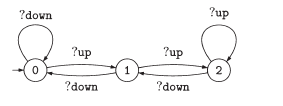
\includegraphics[height=1.5in,width=3.0in]{1_13.png}
    \caption{The cabin}
    \end{figure}
    \begin{figure}
    \centering
    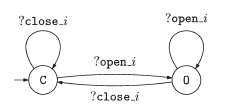
\includegraphics[height=1.5in,width=3.0in]{1_14.png}
    \caption{The $i_{th}$ door}
    \end{figure}
    
    控制器将指令(消息)发送到门和舱室(参见Figure 1.15)。一个更完整的模型将显示控制器如何响应来自电梯用户的请求。状态on i(free i)对应于电梯在第i层的情况,门关闭(门打开)。另外两个状态允许将楼层0与楼层2“直接”联系在一起,即不停留在1层。
    \begin{figure}
    \centering
    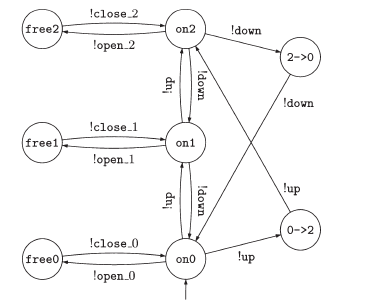
\includegraphics[height=1.5in,width=3.0in]{1_15.png}
    \caption{The controller}
    \end{figure}

    最后,还要确定保持在五个自动机中的每个自动机的每个状态中的基本命题。通常情况下,我们将每个状态都与一个简单的基本属性相关联,简单地对应为状态名。
    
    然后将电梯的自动机建模为这五种自动机的同步积。因此,由此产生的自动机的状态将有五个相应的组件,按照顺序,自动机建模成的状态为door  0、door 1、door 2,cabin和controller。同步约束减少了消息发送/接收的同时执行,正式定义为:
    \begin{tabbing}
      Sync  \kill
      % \> for next tab, \\ for new line...
      Sync=$\{(?open_1,-,-,-,!open_1),(?close_1,-,-,-,!close_1),$\\
     $ \quad(?open_2,-,-,-,!open_2),(?close_2,-,-,-,!close_2)$\\
     $ \quad(?open_3,-,-,-,!open_3),(?close_3,-,-,-,!close_3)$\\
      $\quad(-,-,-,?dowm,!down),(-,-,-,?up,!up)$\}
    \end{tabbing}

    在宣布这个电梯运行之前,我们想要检查一些属性,例如“当舱门在不同楼层的时候,指定楼层的门不能打开”($P_1$),“舱门在打开的时候不能移动”($P_2$)。
    
    对于door 1来说,上面的属性($P_1$)转化为一个事实,即任何以0作为第一个组件的状态都必须是0作为第四个分量。换句话说,我们必须证明没有存在的可达状态是第一个组件是0和第四个组件1或2。请注意,这些事实上是使用原子命题表达的属性。同样的道理也适用于其他的门。
    
    表示属性($P_2$)略显微妙。我们必须证明在任何执行中,前三个组件中的一个是0的状态后面不能有一个第四个组件变化的状态。
    
    模型检查器有能力构建我们的5个自动机的同步积,并自动检查上述属性是否存在。热衷于使用这个电梯的忧心忡忡的读者,可以绕过模型检查器,构建同步的产品,并试图“手工”验证上述属性。
    
    异步消息({\itshape Asynchronous message})。还有一种交换消息的方式:异步通信。当消息没有立即收时,我们称为异步通信。一般来说,假设发出但尚未接收到的消息仍然存在于一个或多个通信通道中,有时候被称为缓冲区。在那里它们通常以FIFO顺序处理(首先是先出):消息是按它们发出的顺序转发的。
    
    例如,这个模型非常适合描述通信协议,而同步通信非常适合描述控制/命令系统。
    
    请注意,痛道通信可以直接用同步通信来理解。它可以包含一个代表通道行为的自动机(或变量)。从$\mathcal{A}$到$\mathcal{A'}$的发送操作,会变成$\mathcal{A}$和通道之间的同步交换,随后是通道与$\mathcal{A'}$之间的同步交换。
    
    如果通信信道是无界的(它可能包含任意数量的消息等待接收),那么可达图是无限的。
    
    如果通道是有界的,可到达图可能具有指数大小(就初始自动机的大小而言)。

    \section{利用共享变量同步(Synchronization by Shared variables)}
    另一种让系统的组件相互通通信的方法是共享一定数量的变量。即使从理论的角度来看,使用一个同步积来标识共享的变量是可能的,但他们的实际兴趣是这样的,我们更倾向于明确地介绍它们。我们之前看到了变量如何“添加”到自动机中。然后,很自然地允许一个(或多个)变量被多个自动机共享。

    再考虑一下两个用户A和B共享打印机的情况。他们与来自1.3节的不公平的打印机管理器的不愉快的经历促使他们决定分享一个变量turn,跟踪谁拥有打印的权利。
    
    因此,用户A以Figure 1.16的自动机建模。描述用户B行为的自动机当然也是对称的(参见Figure 1.17)。
    \begin{figure}
    \centering
    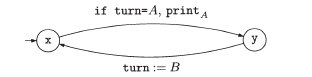
\includegraphics[height=1in,width=3.0in]{1_16.png}
    \caption{The user A}
    \end{figure}
    \begin{figure}
    \centering
    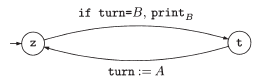
\includegraphics[height=1in,width=3.0in]{1_17.png}
    \caption{The user B}
    \end{figure}

    描述一个包含用户A和用户B地系统全局自动机是由这两个自动机和共享变量的值组成的。如果turn的初始值是A,那么全局自动机的初始状态将是(x,z,A)。从这个状态出发,唯一可能到达的转化是(x,z,B),然后(x,t,B),最后(x,z,A)。如Figure 1.18所示,我们获得了一个全局自动机。
    注意,转化守卫已经消失了,因为我们只考虑了与共享变量的值相一致的转换。
    \begin{figure}
    \centering
    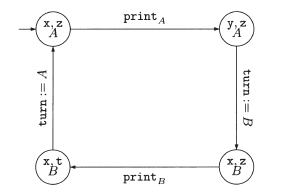
\includegraphics[height=2in,width=3.0in]{1_18.png}
    \caption{A and B resolve conflicts on their own}
    \end{figure}

    给一个带有共享变量的全局自动机下定义当然是可以的。我们不会在这里拼写出这个定义,因为它很自然地把同步积和展开自动机组合起来,而这些概念都已经定义好了。我们只需在打印机用户的示例上演示共享变量构造。
    
    显然,两个用户实现的简单协议保证了没有形如(y,t,-)的状态是可达的。用户确信他们永远不会同时打印。但是他们的协议禁止用户连续打印两次!
    在第一章中,我们以一个更有意义的互斥协议为例。我们仍在努力为我们的两个用户提供一个具有合适的打印机管理策略的共享打印机。我们提出了一个Peterson[Pet81]提出的简化版的算法。
    
    这两个用户现在决定共享3个变量:
    ·变量$r_A$(请求“请求”),当用户希望打印时,将其设置为true。最初rA是假的;
    ·类似地,$r_B$为用户B扮演相应的角色;
    ·再一次用$turn$变量来解决冲突。
    
    Figure 1.19显示了用户A行为的自动机模型(B是对称的,简单地交换A和B的角色),就像在电梯的例子中,我们将每个状态与它的名称对应的唯一的基本命题联系在一起。属性“处于状态4”对应于相应用户的文档打印。
    \begin{figure}
    \centering
    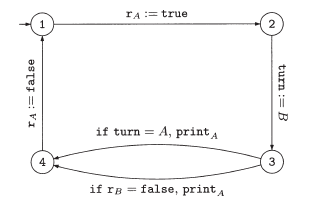
\includegraphics[height=2in,width=3.0in]{1_19.png}
    \caption{Peterson's user A}
    \end{figure}

    这个自动机因此由这两个自动机和三个共享变量$r_A$,$r_B$和$turn$建模而成。一个状态是一个按照那个顺序形成的元组。在这个顺序中,它是A的自动机状态,B的自动机状态,$r_A$的值,$r_B$的值,以及$turn$的值。这个自动机有4 x 4 x 2 x 2 = 128个状态。事实上,可到达的国家只有状态个。特别地,我们可以显示(或请一个模型检查器显示)形如(4、4、-、-)的状态是可访问的,以这种方式保证两个用户不能同时打印。

    实际上,由我们的自动机建模的算法具有我们所追求的所有属性。它特别确保任何打印请求最终都实现了。

    为了证明这种性质,我们必须首先用基本命题来表达它。这正是我们将要定义的各种逻辑的目标。


\end{document} 